\documentclass[1p]{elsarticle_modified}
%\bibliographystyle{elsarticle-num}

%\usepackage[colorlinks]{hyperref}
%\usepackage{abbrmath_seonhwa} %\Abb, \Ascr, \Acal ,\Abf, \Afrak
\usepackage{amsfonts}
\usepackage{amssymb}
\usepackage{amsmath}
\usepackage{amsthm}
\usepackage{scalefnt}
\usepackage{amsbsy}
\usepackage{kotex}
\usepackage{caption}
\usepackage{subfig}
\usepackage{color}
\usepackage{graphicx}
\usepackage{xcolor} %% white, black, red, green, blue, cyan, magenta, yellow
\usepackage{float}
\usepackage{setspace}
\usepackage{hyperref}

\usepackage{tikz}
\usetikzlibrary{arrows}

\usepackage{multirow}
\usepackage{array} % fixed length table
\usepackage{hhline}

%%%%%%%%%%%%%%%%%%%%%
\makeatletter
\renewcommand*\env@matrix[1][\arraystretch]{%
	\edef\arraystretch{#1}%
	\hskip -\arraycolsep
	\let\@ifnextchar\new@ifnextchar
	\array{*\c@MaxMatrixCols c}}
\makeatother %https://tex.stackexchange.com/questions/14071/how-can-i-increase-the-line-spacing-in-a-matrix
%%%%%%%%%%%%%%%

\usepackage[normalem]{ulem}

\newcommand{\msout}[1]{\ifmmode\text{\sout{\ensuremath{#1}}}\else\sout{#1}\fi}
%SOURCE: \msout is \stkout macro in https://tex.stackexchange.com/questions/20609/strikeout-in-math-mode

\newcommand{\cancel}[1]{
	\ifmmode
	{\color{red}\msout{#1}}
	\else
	{\color{red}\sout{#1}}
	\fi
}

\newcommand{\add}[1]{
	{\color{blue}\uwave{#1}}
}

\newcommand{\replace}[2]{
	\ifmmode
	{\color{red}\msout{#1}}{\color{blue}\uwave{#2}}
	\else
	{\color{red}\sout{#1}}{\color{blue}\uwave{#2}}
	\fi
}

\newcommand{\Sol}{\mathcal{S}} %segment
\newcommand{\D}{D} %diagram
\newcommand{\A}{\mathcal{A}} %arc


%%%%%%%%%%%%%%%%%%%%%%%%%%%%%5 test

\def\sl{\operatorname{\textup{SL}}(2,\Cbb)}
\def\psl{\operatorname{\textup{PSL}}(2,\Cbb)}
\def\quan{\mkern 1mu \triangleright \mkern 1mu}

\theoremstyle{definition}
\newtheorem{thm}{Theorem}[section]
\newtheorem{prop}[thm]{Proposition}
\newtheorem{lem}[thm]{Lemma}
\newtheorem{ques}[thm]{Question}
\newtheorem{cor}[thm]{Corollary}
\newtheorem{defn}[thm]{Definition}
\newtheorem{exam}[thm]{Example}
\newtheorem{rmk}[thm]{Remark}
\newtheorem{alg}[thm]{Algorithm}

\newcommand{\I}{\sqrt{-1}}
\begin{document}

%\begin{frontmatter}
%
%\title{Boundary parabolic representations of knots up to 8 crossings}
%
%%% Group authors per affiliation:
%\author{Yunhi Cho} 
%\address{Department of Mathematics, University of Seoul, Seoul, Korea}
%\ead{yhcho@uos.ac.kr}
%
%
%\author{Seonhwa Kim} %\fnref{s_kim}}
%\address{Center for Geometry and Physics, Institute for Basic Science, Pohang, 37673, Korea}
%\ead{ryeona17@ibs.re.kr}
%
%\author{Hyuk Kim}
%\address{Department of Mathematical Sciences, Seoul National University, Seoul 08826, Korea}
%\ead{hyukkim@snu.ac.kr}
%
%\author{Seokbeom Yoon}
%\address{Department of Mathematical Sciences, Seoul National University, Seoul, 08826,  Korea}
%\ead{sbyoon15@snu.ac.kr}
%
%\begin{abstract}
%We find all boundary parabolic representation of knots up to 8 crossings.
%
%\end{abstract}
%\begin{keyword}
%    \MSC[2010] 57M25 
%\end{keyword}
%
%\end{frontmatter}

%\linenumbers
%\tableofcontents
%
\newcommand\colored[1]{\textcolor{white}{\rule[-0.35ex]{0.8em}{1.4ex}}\kern-0.8em\color{red} #1}%
%\newcommand\colored[1]{\textcolor{white}{ #1}\kern-2.17ex	\textcolor{white}{ #1}\kern-1.81ex	\textcolor{white}{ #1}\kern-2.15ex\color{red}#1	}

{\Large $\underline{12n_{0207}~(K12n_{0207})}$}

\setlength{\tabcolsep}{10pt}
\renewcommand{\arraystretch}{1.6}
\vspace{1cm}\begin{tabular}{m{100pt}>{\centering\arraybackslash}m{274pt}}
\multirow{5}{120pt}{
	\centering
	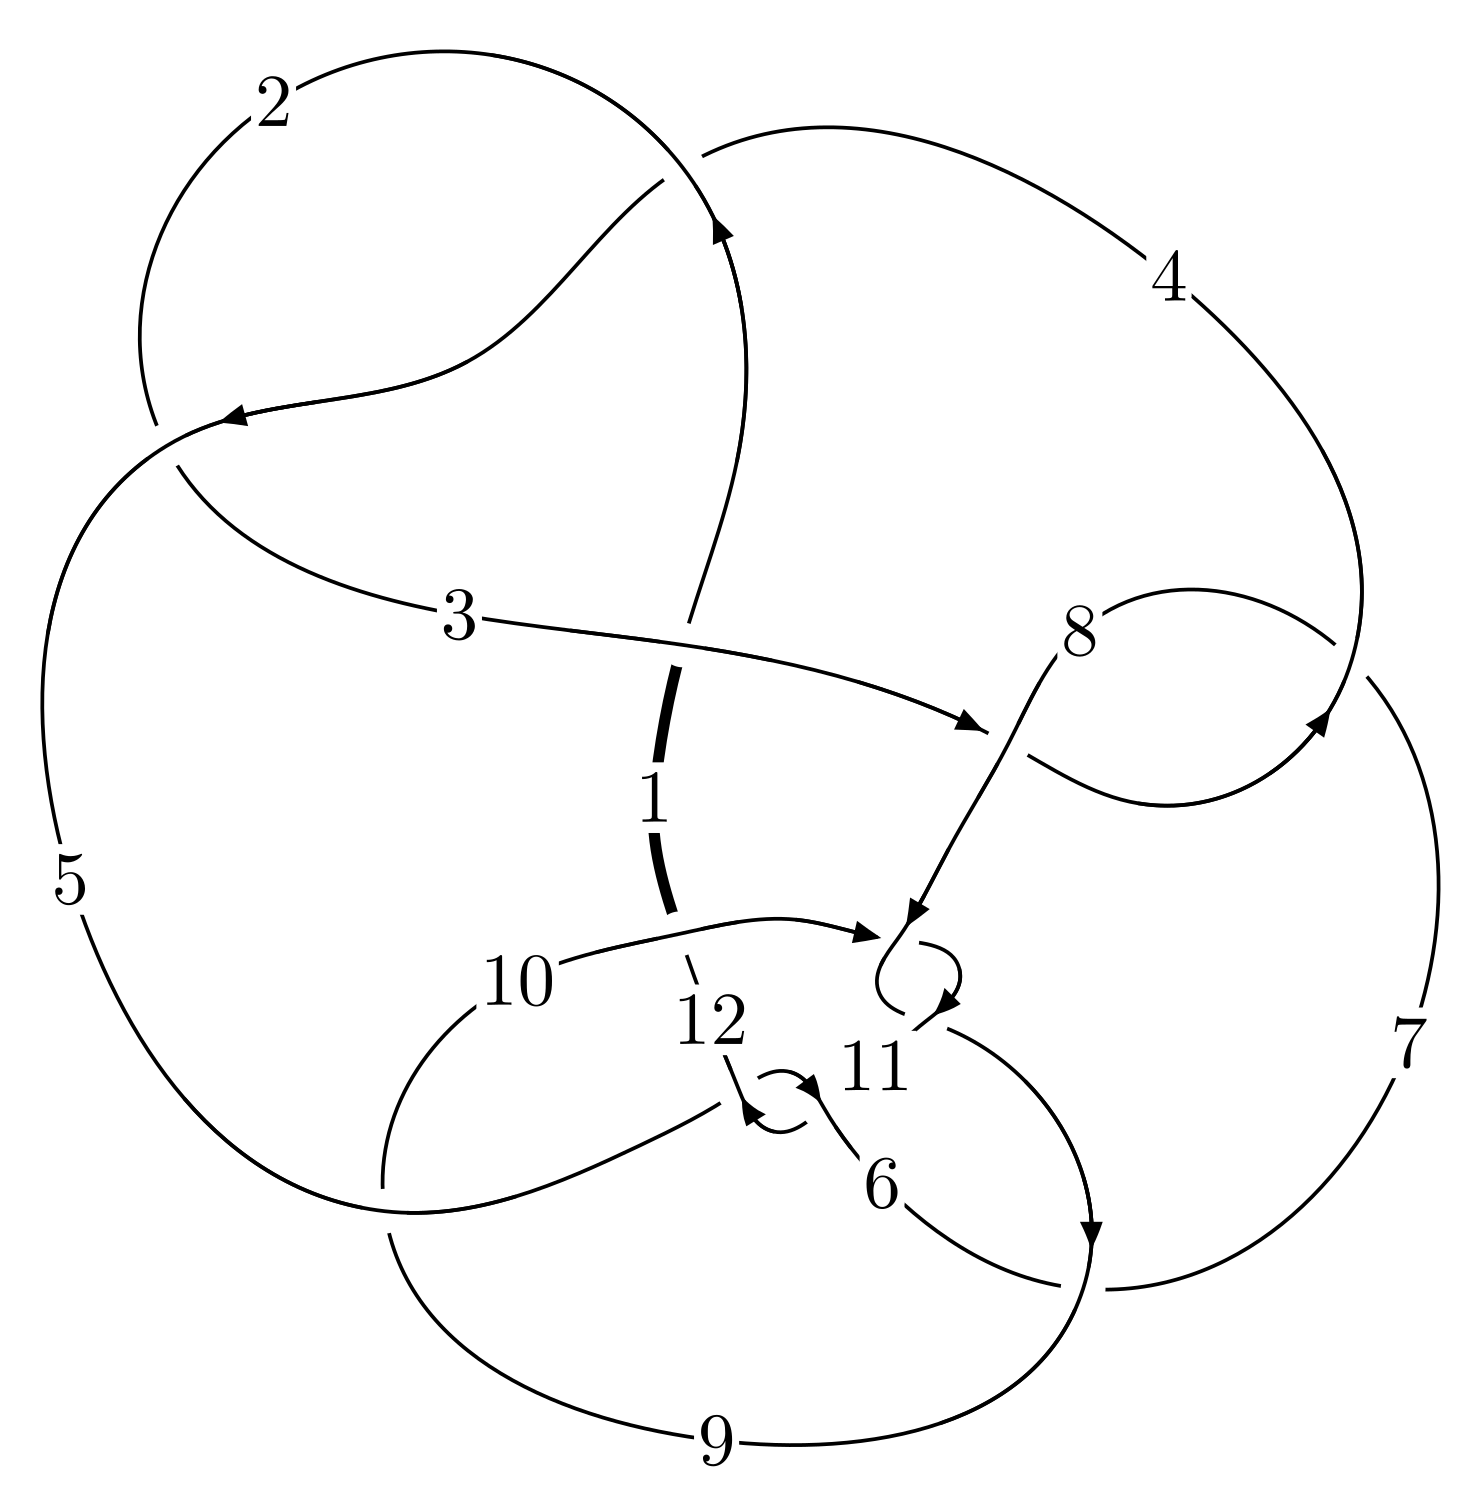
\includegraphics[width=112pt]{../../../GIT/diagram.site/Diagrams/png/2296_12n_0207.png}\\
\ \ \ A knot diagram\footnotemark}&
\allowdisplaybreaks
\textbf{Linearized knot diagam} \\
\cline{2-2}
 &
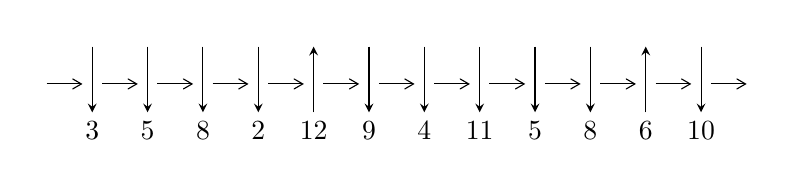
\begin{tikzpicture}[x=20pt, y=17pt]
	% nodes
	\node (C0) at (0, 0) {};
	\node (C1) at (1, 0) {};
	\node (C1U) at (1, +1) {};
	\node (C1D) at (1, -1) {3};

	\node (C2) at (2, 0) {};
	\node (C2U) at (2, +1) {};
	\node (C2D) at (2, -1) {5};

	\node (C3) at (3, 0) {};
	\node (C3U) at (3, +1) {};
	\node (C3D) at (3, -1) {8};

	\node (C4) at (4, 0) {};
	\node (C4U) at (4, +1) {};
	\node (C4D) at (4, -1) {2};

	\node (C5) at (5, 0) {};
	\node (C5U) at (5, +1) {};
	\node (C5D) at (5, -1) {12};

	\node (C6) at (6, 0) {};
	\node (C6U) at (6, +1) {};
	\node (C6D) at (6, -1) {9};

	\node (C7) at (7, 0) {};
	\node (C7U) at (7, +1) {};
	\node (C7D) at (7, -1) {4};

	\node (C8) at (8, 0) {};
	\node (C8U) at (8, +1) {};
	\node (C8D) at (8, -1) {11};

	\node (C9) at (9, 0) {};
	\node (C9U) at (9, +1) {};
	\node (C9D) at (9, -1) {5};

	\node (C10) at (10, 0) {};
	\node (C10U) at (10, +1) {};
	\node (C10D) at (10, -1) {8};

	\node (C11) at (11, 0) {};
	\node (C11U) at (11, +1) {};
	\node (C11D) at (11, -1) {6};

	\node (C12) at (12, 0) {};
	\node (C12U) at (12, +1) {};
	\node (C12D) at (12, -1) {10};
	\node (C13) at (13, 0) {};

	% arrows
	\draw[->,>={angle 60}]
	(C0) edge (C1) (C1) edge (C2) (C2) edge (C3) (C3) edge (C4) (C4) edge (C5) (C5) edge (C6) (C6) edge (C7) (C7) edge (C8) (C8) edge (C9) (C9) edge (C10) (C10) edge (C11) (C11) edge (C12) (C12) edge (C13) ;	\draw[->,>=stealth]
	(C1U) edge (C1D) (C2U) edge (C2D) (C3U) edge (C3D) (C4U) edge (C4D) (C5D) edge (C5U) (C6U) edge (C6D) (C7U) edge (C7D) (C8U) edge (C8D) (C9U) edge (C9D) (C10U) edge (C10D) (C11D) edge (C11U) (C12U) edge (C12D) ;
	\end{tikzpicture} \\
\hhline{~~} \\& 
\textbf{Solving Sequence} \\ \cline{2-2} 
 &
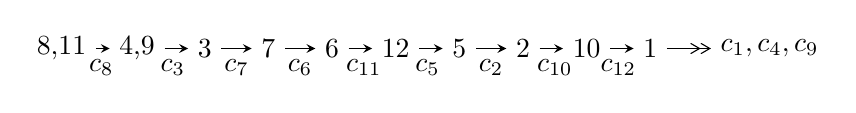
\begin{tikzpicture}[x=23pt, y=7pt]
	% node
	\node (A0) at (-1/8, 0) {8,11};
	\node (A1) at (17/16, 0) {4,9};
	\node (A2) at (17/8, 0) {3};
	\node (A3) at (25/8, 0) {7};
	\node (A4) at (33/8, 0) {6};
	\node (A5) at (41/8, 0) {12};
	\node (A6) at (49/8, 0) {5};
	\node (A7) at (57/8, 0) {2};
	\node (A8) at (65/8, 0) {10};
	\node (A9) at (73/8, 0) {1};
	\node (C1) at (1/2, -1) {$c_{8}$};
	\node (C2) at (13/8, -1) {$c_{3}$};
	\node (C3) at (21/8, -1) {$c_{7}$};
	\node (C4) at (29/8, -1) {$c_{6}$};
	\node (C5) at (37/8, -1) {$c_{11}$};
	\node (C6) at (45/8, -1) {$c_{5}$};
	\node (C7) at (53/8, -1) {$c_{2}$};
	\node (C8) at (61/8, -1) {$c_{10}$};
	\node (C9) at (69/8, -1) {$c_{12}$};
	\node (A10) at (11, 0) {$c_{1},c_{4},c_{9}$};

	% edge
	\draw[->,>=stealth]	
	(A0) edge (A1) (A1) edge (A2) (A2) edge (A3) (A3) edge (A4) (A4) edge (A5) (A5) edge (A6) (A6) edge (A7) (A7) edge (A8) (A8) edge (A9) ;
	\draw[->>,>={angle 60}]	
	(A9) edge (A10);
\end{tikzpicture} \\ 

\end{tabular} \\

\footnotetext{
The image of knot diagram is generated by the software ``\textbf{Draw programme}" developed by Andrew Bartholomew(\url{http://www.layer8.co.uk/maths/draw/index.htm\#Running-draw}), where we modified some parts for our purpose(\url{https://github.com/CATsTAILs/LinksPainter}).
}\phantom \\ \newline 
\centering \textbf{Ideals for irreducible components\footnotemark of $X_{\text{par}}$} 
 
\begin{align*}
I^u_{1}&=\langle 
u^{17}+6 u^{16}+\cdots+b- u,\;u^{15}+6 u^{14}+\cdots+a-2 u,\;u^{18}+7 u^{17}+\cdots+u+1\rangle \\
I^u_{2}&=\langle 
b,\;u^8+2 u^7- u^6-4 u^5- u^4+2 u^3+2 u^2+a+2 u+1,\;u^9+u^8-2 u^7-3 u^6+u^5+3 u^4+2 u^3- u-1\rangle \\
I^u_{3}&=\langle 
-2652 a^8+26713 b+\cdots-65147 a+3162,\;a^9+a^8+2 a^7+19 a^6-5 a^5+15 a^4-6 a^3+4 a^2- a+1,\\
\phantom{I^u_{3}}&\phantom{= \langle  }u-1\rangle \\
I^u_{4}&=\langle 
87 u^{17}+355 u^{16}+\cdots+256 b+153,\;33 u^{17}+85 u^{16}+\cdots+256 a+111,\;u^{18}+4 u^{17}+\cdots-9 u^2+1\rangle \\
\\
\end{align*}
\raggedright * 4 irreducible components of $\dim_{\mathbb{C}}=0$, with total 54 representations.\\
\footnotetext{All coefficients of polynomials are rational numbers. But the coefficients are sometimes approximated in decimal forms when there is not enough margin.}
\newpage
\renewcommand{\arraystretch}{1}
\centering \section*{I. $I^u_{1}= \langle u^{17}+6 u^{16}+\cdots+b- u,\;u^{15}+6 u^{14}+\cdots+a-2 u,\;u^{18}+7 u^{17}+\cdots+u+1 \rangle$}
\flushleft \textbf{(i) Arc colorings}\\
\begin{tabular}{m{7pt} m{180pt} m{7pt} m{180pt} }
\flushright $a_{8}=$&$\begin{pmatrix}1\\0\end{pmatrix}$ \\
\flushright $a_{11}=$&$\begin{pmatrix}0\\u\end{pmatrix}$ \\
\flushright $a_{4}=$&$\begin{pmatrix}- u^{15}-6 u^{14}+\cdots-2 u^2+2 u\\- u^{17}-6 u^{16}+\cdots+4 u^3+u\end{pmatrix}$ \\
\flushright $a_{9}=$&$\begin{pmatrix}1\\u^2\end{pmatrix}$ \\
\flushright $a_{3}=$&$\begin{pmatrix}- u^{17}-6 u^{16}+\cdots-2 u^2+3 u\\- u^{17}-6 u^{16}+\cdots+4 u^3+u\end{pmatrix}$ \\
\flushright $a_{7}=$&$\begin{pmatrix}- u^3-2 u^2+2\\u^3- u\end{pmatrix}$ \\
\flushright $a_{6}=$&$\begin{pmatrix}u^5+2 u^4-4 u^2- u+2\\u^7+2 u^6+u^5-2 u^4- u\end{pmatrix}$ \\
\flushright $a_{12}=$&$\begin{pmatrix}u^{11}+4 u^{10}+4 u^9-8 u^8-18 u^7+24 u^5+8 u^4-15 u^3-4 u^2+4 u\\u^{13}+4 u^{12}+\cdots-2 u^2+u\end{pmatrix}$ \\
\flushright $a_{5}=$&$\begin{pmatrix}u^{17}+6 u^{16}+\cdots- u+2\\u^{17}+7 u^{16}+\cdots- u+1\end{pmatrix}$ \\
\flushright $a_{2}=$&$\begin{pmatrix}-2 u^{17}-13 u^{16}+\cdots+4 u-1\\- u^{17}-7 u^{16}+\cdots+u-1\end{pmatrix}$ \\
\flushright $a_{10}=$&$\begin{pmatrix}u\\u\end{pmatrix}$ \\
\flushright $a_{1}=$&$\begin{pmatrix}- u^{15}-4 u^{14}+\cdots-4 u^2+4 u\\- u^{15}-4 u^{14}+\cdots-2 u^2+u\end{pmatrix}$\\&\end{tabular}
\flushleft \textbf{(ii) Obstruction class $= -1$}\\~\\
\flushleft \textbf{(iii) Cusp Shapes $= -8 u^{17}-56 u^{16}-160 u^{15}-168 u^{14}+176 u^{13}+660 u^{12}+460 u^{11}-492 u^{10}-880 u^9-108 u^8+496 u^7+224 u^6-96 u^5-88 u^4-52 u^3-4 u^2+8 u-2$}\\~\\
\newpage\renewcommand{\arraystretch}{1}
\flushleft \textbf{(iv) u-Polynomials at the component}\newline \\
\begin{tabular}{m{50pt}|m{274pt}}
Crossings & \hspace{64pt}u-Polynomials at each crossing \\
\hline $$\begin{aligned}c_{1}\end{aligned}$$&$\begin{aligned}
&u^{18}+11 u^{17}+\cdots+3 u+1
\end{aligned}$\\
\hline $$\begin{aligned}c_{2},c_{4},c_{8}\\c_{10}\end{aligned}$$&$\begin{aligned}
&u^{18}-7 u^{17}+\cdots- u+1
\end{aligned}$\\
\hline $$\begin{aligned}c_{3},c_{7},c_{9}\end{aligned}$$&$\begin{aligned}
&u^{18}+u^{17}+\cdots+u-1
\end{aligned}$\\
\hline $$\begin{aligned}c_{5},c_{11}\end{aligned}$$&$\begin{aligned}
&u^{18}+u^{17}+\cdots+3 u-1
\end{aligned}$\\
\hline $$\begin{aligned}c_{6}\end{aligned}$$&$\begin{aligned}
&u^{18}-5 u^{17}+\cdots+77 u-23
\end{aligned}$\\
\hline $$\begin{aligned}c_{12}\end{aligned}$$&$\begin{aligned}
&u^{18}-3 u^{17}+\cdots+517 u-1
\end{aligned}$\\
\hline
\end{tabular}\\~\\
\newpage\renewcommand{\arraystretch}{1}
\flushleft \textbf{(v) Riley Polynomials at the component}\newline \\
\begin{tabular}{m{50pt}|m{274pt}}
Crossings & \hspace{64pt}Riley Polynomials at each crossing \\
\hline $$\begin{aligned}c_{1}\end{aligned}$$&$\begin{aligned}
&y^{18}+41 y^{17}+\cdots-47 y+1
\end{aligned}$\\
\hline $$\begin{aligned}c_{2},c_{4},c_{8}\\c_{10}\end{aligned}$$&$\begin{aligned}
&y^{18}-11 y^{17}+\cdots-3 y+1
\end{aligned}$\\
\hline $$\begin{aligned}c_{3},c_{7},c_{9}\end{aligned}$$&$\begin{aligned}
&y^{18}+21 y^{17}+\cdots-7 y+1
\end{aligned}$\\
\hline $$\begin{aligned}c_{5},c_{11}\end{aligned}$$&$\begin{aligned}
&y^{18}+13 y^{17}+\cdots-43 y+1
\end{aligned}$\\
\hline $$\begin{aligned}c_{6}\end{aligned}$$&$\begin{aligned}
&y^{18}+y^{17}+\cdots-5331 y+529
\end{aligned}$\\
\hline $$\begin{aligned}c_{12}\end{aligned}$$&$\begin{aligned}
&y^{18}+29 y^{17}+\cdots-268915 y+1
\end{aligned}$\\
\hline
\end{tabular}\\~\\
\newpage\flushleft \textbf{(vi) Complex Volumes and Cusp Shapes}
$$\begin{array}{c|c|c}  
\text{Solutions to }I^u_{1}& \I (\text{vol} + \sqrt{-1}CS) & \text{Cusp shape}\\
 \hline 
\begin{aligned}
u &= \phantom{-}0.944628\phantom{ +0.000000I} \\
a &= -5.10321\phantom{ +0.000000I} \\
b &= -0.318928\phantom{ +0.000000I}\end{aligned}
 & -3.03100\phantom{ +0.000000I} & -72.2820\phantom{ +0.000000I} \\ \hline\begin{aligned}
u &= \phantom{-}1.090030 + 0.138340 I \\
a &= \phantom{-}0.85982 + 4.45023 I \\
b &= \phantom{-}0.344494 - 0.511075 I\end{aligned}
 & -5.78192 - 0.83339 I & -4.3200 - 13.4737 I \\ \hline\begin{aligned}
u &= \phantom{-}1.090030 - 0.138340 I \\
a &= \phantom{-}0.85982 - 4.45023 I \\
b &= \phantom{-}0.344494 + 0.511075 I\end{aligned}
 & -5.78192 + 0.83339 I & -4.3200 + 13.4737 I \\ \hline\begin{aligned}
u &= -1.074780 + 0.345327 I \\
a &= -0.427778 + 0.032515 I \\
b &= -0.557323 + 0.726879 I\end{aligned}
 & -5.49927 + 7.93492 I & -11.8455 - 13.1993 I \\ \hline\begin{aligned}
u &= -1.074780 - 0.345327 I \\
a &= -0.427778 - 0.032515 I \\
b &= -0.557323 - 0.726879 I\end{aligned}
 & -5.49927 - 7.93492 I & -11.8455 + 13.1993 I \\ \hline\begin{aligned}
u &= -0.771241 + 0.273342 I \\
a &= \phantom{-}0.446361 - 0.431948 I \\
b &= \phantom{-}0.136626 - 0.709955 I\end{aligned}
 & \phantom{-}0.64686 + 2.83787 I & \phantom{-}0.86568 - 9.86296 I \\ \hline\begin{aligned}
u &= -0.771241 - 0.273342 I \\
a &= \phantom{-}0.446361 + 0.431948 I \\
b &= \phantom{-}0.136626 + 0.709955 I\end{aligned}
 & \phantom{-}0.64686 - 2.83787 I & \phantom{-}0.86568 + 9.86296 I \\ \hline\begin{aligned}
u &= \phantom{-}0.681784 + 0.343900 I \\
a &= \phantom{-}0.43124 - 1.72853 I \\
b &= -0.781322 + 0.060789 I\end{aligned}
 & -3.91966 - 2.10303 I & -13.59813 + 2.08848 I \\ \hline\begin{aligned}
u &= \phantom{-}0.681784 - 0.343900 I \\
a &= \phantom{-}0.43124 + 1.72853 I \\
b &= -0.781322 - 0.060789 I\end{aligned}
 & -3.91966 + 2.10303 I & -13.59813 - 2.08848 I \\ \hline\begin{aligned}
u &= \phantom{-}0.466479\phantom{ +0.000000I} \\
a &= -0.766868\phantom{ +0.000000I} \\
b &= \phantom{-}0.604129\phantom{ +0.000000I}\end{aligned}
 & -1.09450\phantom{ +0.000000I} & -7.23730\phantom{ +0.000000I}\\
 \hline 
 \end{array}$$\newpage$$\begin{array}{c|c|c}  
\text{Solutions to }I^u_{1}& \I (\text{vol} + \sqrt{-1}CS) & \text{Cusp shape}\\
 \hline 
\begin{aligned}
u &= -0.123110 + 0.372790 I \\
a &= -1.26837 + 1.31989 I \\
b &= \phantom{-}0.367491 + 0.554636 I\end{aligned}
 & -0.53975 - 1.77290 I & -3.88757 + 3.00933 I \\ \hline\begin{aligned}
u &= -0.123110 - 0.372790 I \\
a &= -1.26837 - 1.31989 I \\
b &= \phantom{-}0.367491 - 0.554636 I\end{aligned}
 & -0.53975 + 1.77290 I & -3.88757 - 3.00933 I \\ \hline\begin{aligned}
u &= -1.28135 + 1.04067 I \\
a &= \phantom{-}0.956293 + 0.739630 I \\
b &= \phantom{-}0.74883 - 1.97520 I\end{aligned}
 & \phantom{-}9.51613 + 3.71804 I & -9.22156 - 1.51475 I \\ \hline\begin{aligned}
u &= -1.28135 - 1.04067 I \\
a &= \phantom{-}0.956293 - 0.739630 I \\
b &= \phantom{-}0.74883 + 1.97520 I\end{aligned}
 & \phantom{-}9.51613 - 3.71804 I & -9.22156 + 1.51475 I \\ \hline\begin{aligned}
u &= -1.33771 + 1.06945 I \\
a &= -0.924080 - 0.832513 I \\
b &= -0.83783 + 2.05810 I\end{aligned}
 & \phantom{-}13.3797 + 9.0997 I & -6.48039 - 4.12934 I \\ \hline\begin{aligned}
u &= -1.33771 - 1.06945 I \\
a &= -0.924080 + 0.832513 I \\
b &= -0.83783 - 2.05810 I\end{aligned}
 & \phantom{-}13.3797 - 9.0997 I & -6.48039 + 4.12934 I \\ \hline\begin{aligned}
u &= -1.38917 + 1.06637 I \\
a &= \phantom{-}0.861553 + 0.883276 I \\
b &= \phantom{-}0.93643 - 2.07951 I\end{aligned}
 & \phantom{-}9.0651 + 14.3484 I & -9.75296 - 6.52825 I \\ \hline\begin{aligned}
u &= -1.38917 - 1.06637 I \\
a &= \phantom{-}0.861553 - 0.883276 I \\
b &= \phantom{-}0.93643 + 2.07951 I\end{aligned}
 & \phantom{-}9.0651 - 14.3484 I & -9.75296 + 6.52825 I\\
 \hline 
 \end{array}$$\newpage\newpage\renewcommand{\arraystretch}{1}
\centering \section*{II. $I^u_{2}= \langle b,\;u^8+2 u^7+\cdots+a+1,\;u^9+u^8-2 u^7-3 u^6+u^5+3 u^4+2 u^3- u-1 \rangle$}
\flushleft \textbf{(i) Arc colorings}\\
\begin{tabular}{m{7pt} m{180pt} m{7pt} m{180pt} }
\flushright $a_{8}=$&$\begin{pmatrix}1\\0\end{pmatrix}$ \\
\flushright $a_{11}=$&$\begin{pmatrix}0\\u\end{pmatrix}$ \\
\flushright $a_{4}=$&$\begin{pmatrix}- u^8-2 u^7+u^6+4 u^5+u^4-2 u^3-2 u^2-2 u-1\\0\end{pmatrix}$ \\
\flushright $a_{9}=$&$\begin{pmatrix}1\\u^2\end{pmatrix}$ \\
\flushright $a_{3}=$&$\begin{pmatrix}- u^8-2 u^7+u^6+4 u^5+u^4-2 u^3-2 u^2-2 u-1\\0\end{pmatrix}$ \\
\flushright $a_{7}=$&$\begin{pmatrix}1\\0\end{pmatrix}$ \\
\flushright $a_{6}=$&$\begin{pmatrix}- u^2+1\\- u^4\end{pmatrix}$ \\
\flushright $a_{12}=$&$\begin{pmatrix}u^5-2 u^3+u\\u^7- u^5+u\end{pmatrix}$ \\
\flushright $a_{5}=$&$\begin{pmatrix}- u^8+3 u^6-3 u^4+1\\- u^8- u^7+3 u^6+2 u^5-3 u^4-2 u^3+1\end{pmatrix}$ \\
\flushright $a_{2}=$&$\begin{pmatrix}-2 u^7-2 u^6+4 u^5+4 u^4-2 u^3-2 u^2-2 u-2\\u^8+u^7-3 u^6-2 u^5+3 u^4+2 u^3-1\end{pmatrix}$ \\
\flushright $a_{10}=$&$\begin{pmatrix}u\\u\end{pmatrix}$ \\
\flushright $a_{1}=$&$\begin{pmatrix}u^8-3 u^6+3 u^4-1\\u^8+u^7-3 u^6-2 u^5+3 u^4+2 u^3-1\end{pmatrix}$\\&\end{tabular}
\flushleft \textbf{(ii) Obstruction class $= 1$}\\~\\
\flushleft \textbf{(iii) Cusp Shapes $= u^8+u^7+2 u^6+u^5-3 u^4-5 u^3+2 u^2+3 u-5$}\\~\\
\newpage\renewcommand{\arraystretch}{1}
\flushleft \textbf{(iv) u-Polynomials at the component}\newline \\
\begin{tabular}{m{50pt}|m{274pt}}
Crossings & \hspace{64pt}u-Polynomials at each crossing \\
\hline $$\begin{aligned}c_{1},c_{2}\end{aligned}$$&$\begin{aligned}
&(u-1)^9
\end{aligned}$\\
\hline $$\begin{aligned}c_{3},c_{7}\end{aligned}$$&$\begin{aligned}
&u^9
\end{aligned}$\\
\hline $$\begin{aligned}c_{4}\end{aligned}$$&$\begin{aligned}
&(u+1)^9
\end{aligned}$\\
\hline $$\begin{aligned}c_{5}\end{aligned}$$&$\begin{aligned}
&u^9+3 u^8+8 u^7+13 u^6+17 u^5+17 u^4+12 u^3+6 u^2+u-1
\end{aligned}$\\
\hline $$\begin{aligned}c_{6}\end{aligned}$$&$\begin{aligned}
&u^9-5 u^8+12 u^7-15 u^6+9 u^5+u^4-4 u^3+2 u^2+u-1
\end{aligned}$\\
\hline $$\begin{aligned}c_{8}\end{aligned}$$&$\begin{aligned}
&u^9+u^8-2 u^7-3 u^6+u^5+3 u^4+2 u^3- u-1
\end{aligned}$\\
\hline $$\begin{aligned}c_{9},c_{12}\end{aligned}$$&$\begin{aligned}
&u^9- u^8+2 u^7- u^6+3 u^5- u^4+2 u^3+u+1
\end{aligned}$\\
\hline $$\begin{aligned}c_{10}\end{aligned}$$&$\begin{aligned}
&u^9- u^8-2 u^7+3 u^6+u^5-3 u^4+2 u^3- u+1
\end{aligned}$\\
\hline $$\begin{aligned}c_{11}\end{aligned}$$&$\begin{aligned}
&u^9-3 u^8+8 u^7-13 u^6+17 u^5-17 u^4+12 u^3-6 u^2+u+1
\end{aligned}$\\
\hline
\end{tabular}\\~\\
\newpage\renewcommand{\arraystretch}{1}
\flushleft \textbf{(v) Riley Polynomials at the component}\newline \\
\begin{tabular}{m{50pt}|m{274pt}}
Crossings & \hspace{64pt}Riley Polynomials at each crossing \\
\hline $$\begin{aligned}c_{1},c_{2},c_{4}\end{aligned}$$&$\begin{aligned}
&(y-1)^9
\end{aligned}$\\
\hline $$\begin{aligned}c_{3},c_{7}\end{aligned}$$&$\begin{aligned}
&y^9
\end{aligned}$\\
\hline $$\begin{aligned}c_{5},c_{11}\end{aligned}$$&$\begin{aligned}
&y^9+7 y^8+20 y^7+25 y^6+5 y^5-15 y^4+22 y^2+13 y-1
\end{aligned}$\\
\hline $$\begin{aligned}c_{6}\end{aligned}$$&$\begin{aligned}
&y^9- y^8+12 y^7-7 y^6+37 y^5+y^4-10 y^2+5 y-1
\end{aligned}$\\
\hline $$\begin{aligned}c_{8},c_{10}\end{aligned}$$&$\begin{aligned}
&y^9-5 y^8+12 y^7-15 y^6+9 y^5+y^4-4 y^3+2 y^2+y-1
\end{aligned}$\\
\hline $$\begin{aligned}c_{9},c_{12}\end{aligned}$$&$\begin{aligned}
&y^9+3 y^8+8 y^7+13 y^6+17 y^5+17 y^4+12 y^3+6 y^2+y-1
\end{aligned}$\\
\hline
\end{tabular}\\~\\
\newpage\flushleft \textbf{(vi) Complex Volumes and Cusp Shapes}
$$\begin{array}{c|c|c}  
\text{Solutions to }I^u_{2}& \I (\text{vol} + \sqrt{-1}CS) & \text{Cusp shape}\\
 \hline 
\begin{aligned}
u &= -0.772920 + 0.510351 I \\
a &= \phantom{-}0.483566 - 0.305056 I \\
b &= \phantom{-0.000000 } 0\end{aligned}
 & \phantom{-}0.13850 + 2.09337 I & -6.02684 - 1.69698 I \\ \hline\begin{aligned}
u &= -0.772920 - 0.510351 I \\
a &= \phantom{-}0.483566 + 0.305056 I \\
b &= \phantom{-0.000000 } 0\end{aligned}
 & \phantom{-}0.13850 - 2.09337 I & -6.02684 + 1.69698 I \\ \hline\begin{aligned}
u &= \phantom{-}0.825933\phantom{ +0.000000I} \\
a &= -3.56378\phantom{ +0.000000I} \\
b &= \phantom{-0.000000 } 0\end{aligned}
 & -2.84338\phantom{ +0.000000I} & -3.87310\phantom{ +0.000000I} \\ \hline\begin{aligned}
u &= \phantom{-}1.173910 + 0.391555 I \\
a &= \phantom{-}1.23246 + 1.62704 I \\
b &= \phantom{-0.000000 } 0\end{aligned}
 & -6.01628 - 1.33617 I & -16.4774 + 4.4812 I \\ \hline\begin{aligned}
u &= \phantom{-}1.173910 - 0.391555 I \\
a &= \phantom{-}1.23246 - 1.62704 I \\
b &= \phantom{-0.000000 } 0\end{aligned}
 & -6.01628 + 1.33617 I & -16.4774 - 4.4812 I \\ \hline\begin{aligned}
u &= -0.141484 + 0.739668 I \\
a &= -1.022450 + 0.246780 I \\
b &= \phantom{-0.000000 } 0\end{aligned}
 & -2.26187 - 2.45442 I & -8.53903 + 2.82066 I \\ \hline\begin{aligned}
u &= -0.141484 - 0.739668 I \\
a &= -1.022450 - 0.246780 I \\
b &= \phantom{-0.000000 } 0\end{aligned}
 & -2.26187 + 2.45442 I & -8.53903 - 2.82066 I \\ \hline\begin{aligned}
u &= -1.172470 + 0.500383 I \\
a &= -0.411691 + 0.129409 I \\
b &= \phantom{-0.000000 } 0\end{aligned}
 & -5.24306 + 7.08493 I & -9.02021 - 2.94778 I \\ \hline\begin{aligned}
u &= -1.172470 - 0.500383 I \\
a &= -0.411691 - 0.129409 I \\
b &= \phantom{-0.000000 } 0\end{aligned}
 & -5.24306 - 7.08493 I & -9.02021 + 2.94778 I\\
 \hline 
 \end{array}$$\newpage\newpage\renewcommand{\arraystretch}{1}
\centering \section*{III. $I^u_{3}= \langle -2652 a^8+26713 b+\cdots-65147 a+3162,\;a^9+a^8+\cdots- a+1,\;u-1 \rangle$}
\flushleft \textbf{(i) Arc colorings}\\
\begin{tabular}{m{7pt} m{180pt} m{7pt} m{180pt} }
\flushright $a_{8}=$&$\begin{pmatrix}1\\0\end{pmatrix}$ \\
\flushright $a_{11}=$&$\begin{pmatrix}0\\1\end{pmatrix}$ \\
\flushright $a_{4}=$&$\begin{pmatrix}a\\0.0992775 a^{8}-0.0110059 a^{7}+\cdots+2.43878 a-0.118369\end{pmatrix}$ \\
\flushright $a_{9}=$&$\begin{pmatrix}1\\1\end{pmatrix}$ \\
\flushright $a_{3}=$&$\begin{pmatrix}0.0992775 a^{8}-0.0110059 a^{7}+\cdots+3.43878 a-0.118369\\0.0992775 a^{8}-0.0110059 a^{7}+\cdots+2.43878 a-0.118369\end{pmatrix}$ \\
\flushright $a_{7}=$&$\begin{pmatrix}0.110283 a^{8}+0.0737469 a^{7}+\cdots+0.0190918 a+1.09928\\0.235690 a^{8}+0.0462696 a^{7}+\cdots-0.0895444 a+0.334369\end{pmatrix}$ \\
\flushright $a_{6}=$&$\begin{pmatrix}0.235690 a^{8}+0.0462696 a^{7}+\cdots-0.0895444 a+0.334369\\0.361098 a^{8}+0.0187923 a^{7}+\cdots-0.198181 a-0.430539\end{pmatrix}$ \\
\flushright $a_{12}=$&$\begin{pmatrix}0.895893 a^{8}+0.647288 a^{7}+\cdots+0.918841 a-1.22203\\1.03171 a^{8}+0.767978 a^{7}+\cdots+1.14806 a-1.23011\end{pmatrix}$ \\
\flushright $a_{5}=$&$\begin{pmatrix}1.32041 a^{8}+1.20204 a^{7}+\cdots+3.01677 a-1.11279\\1.32041 a^{8}+1.20204 a^{7}+\cdots+3.01677 a-1.11279\end{pmatrix}$ \\
\flushright $a_{2}=$&$\begin{pmatrix}1.32041 a^{8}+1.20204 a^{7}+\cdots+4.01677 a-1.11279\\1.32041 a^{8}+1.20204 a^{7}+\cdots+3.01677 a-1.11279\end{pmatrix}$ \\
\flushright $a_{10}=$&$\begin{pmatrix}1\\1\end{pmatrix}$ \\
\flushright $a_{1}=$&$\begin{pmatrix}0.760079 a^{8}+0.526598 a^{7}+\cdots+0.689627 a-1.21394\\0.895893 a^{8}+0.647288 a^{7}+\cdots+0.918841 a-1.22203\end{pmatrix}$\\&\end{tabular}
\flushleft \textbf{(ii) Obstruction class $= 1$}\\~\\
\flushleft \textbf{(iii) Cusp Shapes $= \frac{20687}{26713} a^8+\frac{30282}{26713} a^7+\frac{57293}{26713} a^6+\frac{423871}{26713} a^5+\frac{90930}{26713} a^4+\frac{389154}{26713} a^3+\frac{110924}{26713} a^2-\frac{5178}{26713} a-\frac{181861}{26713}$}\\~\\
\newpage\renewcommand{\arraystretch}{1}
\flushleft \textbf{(iv) u-Polynomials at the component}\newline \\
\begin{tabular}{m{50pt}|m{274pt}}
Crossings & \hspace{64pt}u-Polynomials at each crossing \\
\hline $$\begin{aligned}c_{1}\end{aligned}$$&$\begin{aligned}
&u^9-5 u^8+12 u^7-15 u^6+9 u^5+u^4-4 u^3+2 u^2+u-1
\end{aligned}$\\
\hline $$\begin{aligned}c_{2}\end{aligned}$$&$\begin{aligned}
&u^9+u^8-2 u^7-3 u^6+u^5+3 u^4+2 u^3- u-1
\end{aligned}$\\
\hline $$\begin{aligned}c_{3}\end{aligned}$$&$\begin{aligned}
&u^9+u^8+2 u^7+u^6+3 u^5+u^4+2 u^3+u-1
\end{aligned}$\\
\hline $$\begin{aligned}c_{4}\end{aligned}$$&$\begin{aligned}
&u^9- u^8-2 u^7+3 u^6+u^5-3 u^4+2 u^3- u+1
\end{aligned}$\\
\hline $$\begin{aligned}c_{5}\end{aligned}$$&$\begin{aligned}
&u^9-3 u^8+8 u^7-13 u^6+17 u^5-17 u^4+12 u^3-6 u^2+u+1
\end{aligned}$\\
\hline $$\begin{aligned}c_{6}\end{aligned}$$&$\begin{aligned}
&u^9-2 u^8+5 u^7-22 u^6+52 u^5-63 u^4+41 u^3-10 u^2-2 u+1
\end{aligned}$\\
\hline $$\begin{aligned}c_{7}\end{aligned}$$&$\begin{aligned}
&u^9- u^8+2 u^7- u^6+3 u^5- u^4+2 u^3+u+1
\end{aligned}$\\
\hline $$\begin{aligned}c_{8}\end{aligned}$$&$\begin{aligned}
&(u-1)^9
\end{aligned}$\\
\hline $$\begin{aligned}c_{9}\end{aligned}$$&$\begin{aligned}
&u^9
\end{aligned}$\\
\hline $$\begin{aligned}c_{10}\end{aligned}$$&$\begin{aligned}
&(u+1)^9
\end{aligned}$\\
\hline $$\begin{aligned}c_{11}\end{aligned}$$&$\begin{aligned}
&u^9+3 u^8+8 u^7+13 u^6+17 u^5+17 u^4+12 u^3+6 u^2+u-1
\end{aligned}$\\
\hline $$\begin{aligned}c_{12}\end{aligned}$$&$\begin{aligned}
&u^9-3 u^8+3 u^7+2 u^6+u^5+9 u^4+3 u^3+2 u+1
\end{aligned}$\\
\hline
\end{tabular}\\~\\
\newpage\renewcommand{\arraystretch}{1}
\flushleft \textbf{(v) Riley Polynomials at the component}\newline \\
\begin{tabular}{m{50pt}|m{274pt}}
Crossings & \hspace{64pt}Riley Polynomials at each crossing \\
\hline $$\begin{aligned}c_{1}\end{aligned}$$&$\begin{aligned}
&y^9- y^8+12 y^7-7 y^6+37 y^5+y^4-10 y^2+5 y-1
\end{aligned}$\\
\hline $$\begin{aligned}c_{2},c_{4}\end{aligned}$$&$\begin{aligned}
&y^9-5 y^8+12 y^7-15 y^6+9 y^5+y^4-4 y^3+2 y^2+y-1
\end{aligned}$\\
\hline $$\begin{aligned}c_{3},c_{7}\end{aligned}$$&$\begin{aligned}
&y^9+3 y^8+8 y^7+13 y^6+17 y^5+17 y^4+12 y^3+6 y^2+y-1
\end{aligned}$\\
\hline $$\begin{aligned}c_{5},c_{11}\end{aligned}$$&$\begin{aligned}
&y^9+7 y^8+20 y^7+25 y^6+5 y^5-15 y^4+22 y^2+13 y-1
\end{aligned}$\\
\hline $$\begin{aligned}c_{6}\end{aligned}$$&$\begin{aligned}
&y^9+6 y^8+\cdots+24 y-1
\end{aligned}$\\
\hline $$\begin{aligned}c_{8},c_{10}\end{aligned}$$&$\begin{aligned}
&(y-1)^9
\end{aligned}$\\
\hline $$\begin{aligned}c_{9}\end{aligned}$$&$\begin{aligned}
&y^9
\end{aligned}$\\
\hline $$\begin{aligned}c_{12}\end{aligned}$$&$\begin{aligned}
&y^9-3 y^8+23 y^7+62 y^6-13 y^5-57 y^4+9 y^3-6 y^2+4 y-1
\end{aligned}$\\
\hline
\end{tabular}\\~\\
\newpage\flushleft \textbf{(vi) Complex Volumes and Cusp Shapes}
$$\begin{array}{c|c|c}  
\text{Solutions to }I^u_{3}& \I (\text{vol} + \sqrt{-1}CS) & \text{Cusp shape}\\
 \hline 
\begin{aligned}
u &= \phantom{-}1.00000\phantom{ +0.000000I} \\
a &= -0.037875 + 0.791187 I \\
b &= -0.628449 + 0.875112 I\end{aligned}
 & -2.26187 + 2.45442 I & -8.53903 - 2.82066 I \\ \hline\begin{aligned}
u &= \phantom{-}1.00000\phantom{ +0.000000I} \\
a &= -0.037875 - 0.791187 I \\
b &= -0.628449 - 0.875112 I\end{aligned}
 & -2.26187 - 2.45442 I & -8.53903 + 2.82066 I \\ \hline\begin{aligned}
u &= \phantom{-}1.00000\phantom{ +0.000000I} \\
a &= \phantom{-}0.417942 + 0.357732 I \\
b &= \phantom{-}0.728966 + 0.986295 I\end{aligned}
 & -5.24306 - 7.08493 I & -9.02021 + 2.94778 I \\ \hline\begin{aligned}
u &= \phantom{-}1.00000\phantom{ +0.000000I} \\
a &= \phantom{-}0.417942 - 0.357732 I \\
b &= \phantom{-}0.728966 - 0.986295 I\end{aligned}
 & -5.24306 + 7.08493 I & -9.02021 - 2.94778 I \\ \hline\begin{aligned}
u &= \phantom{-}1.00000\phantom{ +0.000000I} \\
a &= -0.218072 + 0.482572 I \\
b &= -0.140343 + 0.966856 I\end{aligned}
 & \phantom{-}0.13850 + 2.09337 I & -6.02684 - 1.69698 I \\ \hline\begin{aligned}
u &= \phantom{-}1.00000\phantom{ +0.000000I} \\
a &= -0.218072 - 0.482572 I \\
b &= -0.140343 - 0.966856 I\end{aligned}
 & \phantom{-}0.13850 - 2.09337 I & -6.02684 + 1.69698 I \\ \hline\begin{aligned}
u &= \phantom{-}1.00000\phantom{ +0.000000I} \\
a &= \phantom{-}0.80973 + 2.39258 I \\
b &= \phantom{-}0.796005 - 0.733148 I\end{aligned}
 & -6.01628 - 1.33617 I & -16.4774 + 4.4812 I \\ \hline\begin{aligned}
u &= \phantom{-}1.00000\phantom{ +0.000000I} \\
a &= \phantom{-}0.80973 - 2.39258 I \\
b &= \phantom{-}0.796005 + 0.733148 I\end{aligned}
 & -6.01628 + 1.33617 I & -16.4774 - 4.4812 I \\ \hline\begin{aligned}
u &= \phantom{-}1.00000\phantom{ +0.000000I} \\
a &= -2.94345\phantom{ +0.000000I} \\
b &= -0.512358\phantom{ +0.000000I}\end{aligned}
 & -2.84338\phantom{ +0.000000I} & -3.87310\phantom{ +0.000000I}\\
 \hline 
 \end{array}$$\newpage\newpage\renewcommand{\arraystretch}{1}
\centering \section*{IV. $I^u_{4}= \langle 87 u^{17}+355 u^{16}+\cdots+256 b+153,\;33 u^{17}+85 u^{16}+\cdots+256 a+111,\;u^{18}+4 u^{17}+\cdots-9 u^2+1 \rangle$}
\flushleft \textbf{(i) Arc colorings}\\
\begin{tabular}{m{7pt} m{180pt} m{7pt} m{180pt} }
\flushright $a_{8}=$&$\begin{pmatrix}1\\0\end{pmatrix}$ \\
\flushright $a_{11}=$&$\begin{pmatrix}0\\u\end{pmatrix}$ \\
\flushright $a_{4}=$&$\begin{pmatrix}-0.128906 u^{17}-0.332031 u^{16}+\cdots-8.87109 u-0.433594\\-0.339844 u^{17}-1.38672 u^{16}+\cdots+1.46484 u-0.597656\end{pmatrix}$ \\
\flushright $a_{9}=$&$\begin{pmatrix}1\\u^2\end{pmatrix}$ \\
\flushright $a_{3}=$&$\begin{pmatrix}-0.468750 u^{17}-1.71875 u^{16}+\cdots-7.40625 u-1.03125\\-0.339844 u^{17}-1.38672 u^{16}+\cdots+1.46484 u-0.597656\end{pmatrix}$ \\
\flushright $a_{7}=$&$\begin{pmatrix}-0.0507813 u^{17}-0.160156 u^{16}+\cdots-5.93359 u+2.94141\\-0.226563 u^{17}-0.765625 u^{16}+\cdots-3.55469 u-0.328125\end{pmatrix}$ \\
\flushright $a_{6}=$&$\begin{pmatrix}-0.242188 u^{17}-0.812500 u^{16}+\cdots-9.53906 u+2.65625\\-0.277344 u^{17}-0.964844 u^{16}+\cdots-3.36328 u-0.441406\end{pmatrix}$ \\
\flushright $a_{12}=$&$\begin{pmatrix}0.812500 u^{17}+3.19531 u^{16}+\cdots-0.437500 u+3.36719\\0.0351563 u^{17}+0.121094 u^{16}+\cdots-4.28516 u+1.14453\end{pmatrix}$ \\
\flushright $a_{5}=$&$\begin{pmatrix}0.128906 u^{17}+0.332031 u^{16}+\cdots+8.87109 u+0.433594\\0.183594 u^{17}+0.667969 u^{16}+\cdots-0.433594 u+0.128906\end{pmatrix}$ \\
\flushright $a_{2}=$&$\begin{pmatrix}0\\-0.183594 u^{17}-0.667969 u^{16}+\cdots+0.433594 u-0.128906\end{pmatrix}$ \\
\flushright $a_{10}=$&$\begin{pmatrix}u\\u\end{pmatrix}$ \\
\flushright $a_{1}=$&$\begin{pmatrix}0.714844 u^{17}+2.70703 u^{16}+\cdots-1.21484 u+3.40234\\-0.0625000 u^{17}-0.367188 u^{16}+\cdots-5.06250 u+1.17969\end{pmatrix}$\\&\end{tabular}
\flushleft \textbf{(ii) Obstruction class $= -1$}\\~\\
\flushleft \textbf{(iii) Cusp Shapes $= -\frac{43}{128} u^{17}-\frac{91}{64} u^{16}+\cdots+\frac{75}{128} u-\frac{619}{64}$}\\~\\
\newpage\renewcommand{\arraystretch}{1}
\flushleft \textbf{(iv) u-Polynomials at the component}\newline \\
\begin{tabular}{m{50pt}|m{274pt}}
Crossings & \hspace{64pt}u-Polynomials at each crossing \\
\hline $$\begin{aligned}c_{1}\end{aligned}$$&$\begin{aligned}
&u^{18}-10 u^{17}+\cdots+18 u+1
\end{aligned}$\\
\hline $$\begin{aligned}c_{2},c_{4},c_{8}\\c_{10}\end{aligned}$$&$\begin{aligned}
&u^{18}-4 u^{17}+\cdots-9 u^2+1
\end{aligned}$\\
\hline $$\begin{aligned}c_{3},c_{7},c_{9}\end{aligned}$$&$\begin{aligned}
&u^{18}+u^{17}+\cdots+1024 u+512
\end{aligned}$\\
\hline $$\begin{aligned}c_{5},c_{11}\end{aligned}$$&$\begin{aligned}
&(u^9+u^8+4 u^7+3 u^6+5 u^5+3 u^4-3 u-1)^2
\end{aligned}$\\
\hline $$\begin{aligned}c_{6}\end{aligned}$$&$\begin{aligned}
&u^{18}-3 u^{17}+\cdots+3241 u+1303
\end{aligned}$\\
\hline $$\begin{aligned}c_{12}\end{aligned}$$&$\begin{aligned}
&u^{18}+4 u^{17}+\cdots+1179 u-199
\end{aligned}$\\
\hline
\end{tabular}\\~\\
\newpage\renewcommand{\arraystretch}{1}
\flushleft \textbf{(v) Riley Polynomials at the component}\newline \\
\begin{tabular}{m{50pt}|m{274pt}}
Crossings & \hspace{64pt}Riley Polynomials at each crossing \\
\hline $$\begin{aligned}c_{1}\end{aligned}$$&$\begin{aligned}
&y^{18}+38 y^{17}+\cdots-206 y+1
\end{aligned}$\\
\hline $$\begin{aligned}c_{2},c_{4},c_{8}\\c_{10}\end{aligned}$$&$\begin{aligned}
&y^{18}+10 y^{17}+\cdots-18 y+1
\end{aligned}$\\
\hline $$\begin{aligned}c_{3},c_{7},c_{9}\end{aligned}$$&$\begin{aligned}
&y^{18}+39 y^{17}+\cdots-262144 y+262144
\end{aligned}$\\
\hline $$\begin{aligned}c_{5},c_{11}\end{aligned}$$&$\begin{aligned}
&(y^9+7 y^8+20 y^7+25 y^6+y^5-31 y^4-24 y^3+6 y^2+9 y-1)^2
\end{aligned}$\\
\hline $$\begin{aligned}c_{6}\end{aligned}$$&$\begin{aligned}
&y^{18}+33 y^{17}+\cdots-7027677 y+1697809
\end{aligned}$\\
\hline $$\begin{aligned}c_{12}\end{aligned}$$&$\begin{aligned}
&y^{18}+40 y^{17}+\cdots-5352529 y+39601
\end{aligned}$\\
\hline
\end{tabular}\\~\\
\newpage\flushleft \textbf{(vi) Complex Volumes and Cusp Shapes}
$$\begin{array}{c|c|c}  
\text{Solutions to }I^u_{4}& \I (\text{vol} + \sqrt{-1}CS) & \text{Cusp shape}\\
 \hline 
\begin{aligned}
u &= -0.292342 + 0.889650 I \\
a &= \phantom{-}0.150415 + 1.204670 I \\
b &= \phantom{-}1.52260 - 1.29705 I\end{aligned}
 & \phantom{-}0.11314 + 3.86354 I & -7.87583 - 4.20503 I \\ \hline\begin{aligned}
u &= -0.292342 - 0.889650 I \\
a &= \phantom{-}0.150415 - 1.204670 I \\
b &= \phantom{-}1.52260 + 1.29705 I\end{aligned}
 & \phantom{-}0.11314 - 3.86354 I & -7.87583 + 4.20503 I \\ \hline\begin{aligned}
u &= -0.167320 + 1.143090 I \\
a &= -0.144832 - 0.989456 I \\
b &= -0.96197 + 1.32057 I\end{aligned}
 & \phantom{-}3.85626\phantom{ +0.000000I} & -3.50861 + 0. I\phantom{ +0.000000I} \\ \hline\begin{aligned}
u &= -0.167320 - 1.143090 I \\
a &= -0.144832 + 0.989456 I \\
b &= -0.96197 - 1.32057 I\end{aligned}
 & \phantom{-}3.85626\phantom{ +0.000000I} & -3.50861 + 0. I\phantom{ +0.000000I} \\ \hline\begin{aligned}
u &= \phantom{-}0.673526\phantom{ +0.000000I} \\
a &= -0.538185\phantom{ +0.000000I} \\
b &= \phantom{-}0.433195\phantom{ +0.000000I}\end{aligned}
 & -1.08370\phantom{ +0.000000I} & -8.12940\phantom{ +0.000000I} \\ \hline\begin{aligned}
u &= \phantom{-}1.255930 + 0.512460 I \\
a &= \phantom{-}0.105046 - 0.414131 I \\
b &= -0.200843 + 0.459012 I\end{aligned}
 & -4.49282 - 1.55423 I & -10.08319 + 1.78109 I \\ \hline\begin{aligned}
u &= \phantom{-}1.255930 - 0.512460 I \\
a &= \phantom{-}0.105046 + 0.414131 I \\
b &= -0.200843 - 0.459012 I\end{aligned}
 & -4.49282 + 1.55423 I & -10.08319 - 1.78109 I \\ \hline\begin{aligned}
u &= \phantom{-}0.095228 + 1.376890 I \\
a &= \phantom{-}0.102057 + 0.817363 I \\
b &= \phantom{-}0.595275 - 1.147110 I\end{aligned}
 & \phantom{-}0.11314 - 3.86354 I & -7.87583 + 4.20503 I \\ \hline\begin{aligned}
u &= \phantom{-}0.095228 - 1.376890 I \\
a &= \phantom{-}0.102057 - 0.817363 I \\
b &= \phantom{-}0.595275 + 1.147110 I\end{aligned}
 & \phantom{-}0.11314 + 3.86354 I & -7.87583 - 4.20503 I \\ \hline\begin{aligned}
u &= -1.04620 + 1.32365 I \\
a &= -0.622785 - 0.838280 I \\
b &= \phantom{-}0.01330 + 2.66058 I\end{aligned}
 & \phantom{-}10.52390 + 4.99486 I & -8.55415 - 3.07435 I\\
 \hline 
 \end{array}$$\newpage$$\begin{array}{c|c|c}  
\text{Solutions to }I^u_{4}& \I (\text{vol} + \sqrt{-1}CS) & \text{Cusp shape}\\
 \hline 
\begin{aligned}
u &= -1.04620 - 1.32365 I \\
a &= -0.622785 + 0.838280 I \\
b &= \phantom{-}0.01330 - 2.66058 I\end{aligned}
 & \phantom{-}10.52390 - 4.99486 I & -8.55415 + 3.07435 I \\ \hline\begin{aligned}
u &= -0.156952 + 0.191508 I \\
a &= \phantom{-}0.57547 - 2.26873 I \\
b &= -1.015350 - 0.875548 I\end{aligned}
 & -4.49282 + 1.55423 I & -10.08319 - 1.78109 I \\ \hline\begin{aligned}
u &= -0.156952 - 0.191508 I \\
a &= \phantom{-}0.57547 + 2.26873 I \\
b &= -1.015350 + 0.875548 I\end{aligned}
 & -4.49282 - 1.55423 I & -10.08319 + 1.78109 I \\ \hline\begin{aligned}
u &= -1.06998 + 1.41248 I \\
a &= \phantom{-}0.603827 + 0.797115 I \\
b &= -0.12400 - 2.50290 I\end{aligned}
 & \phantom{-}14.5478\phantom{ +0.000000I} & -5.33565 + 0. I\phantom{ +0.000000I} \\ \hline\begin{aligned}
u &= -1.06998 - 1.41248 I \\
a &= \phantom{-}0.603827 - 0.797115 I \\
b &= -0.12400 + 2.50290 I\end{aligned}
 & \phantom{-}14.5478\phantom{ +0.000000I} & -5.33565 + 0. I\phantom{ +0.000000I} \\ \hline\begin{aligned}
u &= \phantom{-}0.195082\phantom{ +0.000000I} \\
a &= -1.85810\phantom{ +0.000000I} \\
b &= \phantom{-}0.606622\phantom{ +0.000000I}\end{aligned}
 & -1.08370\phantom{ +0.000000I} & -8.12940\phantom{ +0.000000I} \\ \hline\begin{aligned}
u &= -1.05267 + 1.50913 I \\
a &= -0.571061 - 0.768659 I \\
b &= \phantom{-}0.15107 + 2.32872 I\end{aligned}
 & \phantom{-}10.52390 - 4.99486 I & -8.55415 + 3.07435 I \\ \hline\begin{aligned}
u &= -1.05267 - 1.50913 I \\
a &= -0.571061 + 0.768659 I \\
b &= \phantom{-}0.15107 - 2.32872 I\end{aligned}
 & \phantom{-}10.52390 + 4.99486 I & -8.55415 - 3.07435 I\\
 \hline 
 \end{array}$$\newpage
\newpage\renewcommand{\arraystretch}{1}
\centering \section*{ V. u-Polynomials}
\begin{tabular}{m{50pt}|m{274pt}}
Crossings & \hspace{64pt}u-Polynomials at each crossing \\
\hline $$\begin{aligned}c_{1}\end{aligned}$$&$\begin{aligned}
&(u-1)^9(u^9-5 u^8+12 u^7-15 u^6+9 u^5+u^4-4 u^3+2 u^2+u-1)\\
&\cdot(u^{18}-10 u^{17}+\cdots+18 u+1)(u^{18}+11 u^{17}+\cdots+3 u+1)
\end{aligned}$\\
\hline $$\begin{aligned}c_{2},c_{8}\end{aligned}$$&$\begin{aligned}
&(u-1)^9(u^9+u^8-2 u^7-3 u^6+u^5+3 u^4+2 u^3- u-1)\\
&\cdot(u^{18}-7 u^{17}+\cdots- u+1)(u^{18}-4 u^{17}+\cdots-9 u^2+1)
\end{aligned}$\\
\hline $$\begin{aligned}c_{3}\end{aligned}$$&$\begin{aligned}
&u^9(u^9+u^8+\cdots+u-1)(u^{18}+u^{17}+\cdots+u-1)\\
&\cdot(u^{18}+u^{17}+\cdots+1024 u+512)
\end{aligned}$\\
\hline $$\begin{aligned}c_{4},c_{10}\end{aligned}$$&$\begin{aligned}
&(u+1)^9(u^9- u^8-2 u^7+3 u^6+u^5-3 u^4+2 u^3- u+1)\\
&\cdot(u^{18}-7 u^{17}+\cdots- u+1)(u^{18}-4 u^{17}+\cdots-9 u^2+1)
\end{aligned}$\\
\hline $$\begin{aligned}c_{5},c_{11}\end{aligned}$$&$\begin{aligned}
&(u^9-3 u^8+8 u^7-13 u^6+17 u^5-17 u^4+12 u^3-6 u^2+u+1)\\
&\cdot(u^9+u^8+4 u^7+3 u^6+5 u^5+3 u^4-3 u-1)^2\\
&\cdot(u^9+3 u^8+8 u^7+13 u^6+17 u^5+17 u^4+12 u^3+6 u^2+u-1)\\
&\cdot(u^{18}+u^{17}+\cdots+3 u-1)
\end{aligned}$\\
\hline $$\begin{aligned}c_{6}\end{aligned}$$&$\begin{aligned}
&(u^9-5 u^8+12 u^7-15 u^6+9 u^5+u^4-4 u^3+2 u^2+u-1)\\
&\cdot(u^9-2 u^8+5 u^7-22 u^6+52 u^5-63 u^4+41 u^3-10 u^2-2 u+1)\\
&\cdot(u^{18}-5 u^{17}+\cdots+77 u-23)(u^{18}-3 u^{17}+\cdots+3241 u+1303)
\end{aligned}$\\
\hline $$\begin{aligned}c_{7},c_{9}\end{aligned}$$&$\begin{aligned}
&u^9(u^9- u^8+\cdots+u+1)(u^{18}+u^{17}+\cdots+u-1)\\
&\cdot(u^{18}+u^{17}+\cdots+1024 u+512)
\end{aligned}$\\
\hline $$\begin{aligned}c_{12}\end{aligned}$$&$\begin{aligned}
&(u^9-3 u^8+3 u^7+2 u^6+u^5+9 u^4+3 u^3+2 u+1)\\
&\cdot(u^9- u^8+2 u^7- u^6+3 u^5- u^4+2 u^3+u+1)\\
&\cdot(u^{18}-3 u^{17}+\cdots+517 u-1)(u^{18}+4 u^{17}+\cdots+1179 u-199)
\end{aligned}$\\
\hline
\end{tabular}\newpage\renewcommand{\arraystretch}{1}
\centering \section*{ VI. Riley Polynomials}
\begin{tabular}{m{50pt}|m{274pt}}
Crossings & \hspace{64pt}Riley Polynomials at each crossing \\
\hline $$\begin{aligned}c_{1}\end{aligned}$$&$\begin{aligned}
&(y-1)^9(y^9- y^8+12 y^7-7 y^6+37 y^5+y^4-10 y^2+5 y-1)\\
&\cdot(y^{18}+38 y^{17}+\cdots-206 y+1)(y^{18}+41 y^{17}+\cdots-47 y+1)
\end{aligned}$\\
\hline $$\begin{aligned}c_{2},c_{4},c_{8}\\c_{10}\end{aligned}$$&$\begin{aligned}
&(y-1)^9(y^9-5 y^8+12 y^7-15 y^6+9 y^5+y^4-4 y^3+2 y^2+y-1)\\
&\cdot(y^{18}-11 y^{17}+\cdots-3 y+1)(y^{18}+10 y^{17}+\cdots-18 y+1)
\end{aligned}$\\
\hline $$\begin{aligned}c_{3},c_{7},c_{9}\end{aligned}$$&$\begin{aligned}
&y^9(y^9+3 y^8+8 y^7+13 y^6+17 y^5+17 y^4+12 y^3+6 y^2+y-1)\\
&\cdot(y^{18}+21 y^{17}+\cdots-7 y+1)(y^{18}+39 y^{17}+\cdots-262144 y+262144)
\end{aligned}$\\
\hline $$\begin{aligned}c_{5},c_{11}\end{aligned}$$&$\begin{aligned}
&(y^9+7 y^8+20 y^7+25 y^6+y^5-31 y^4-24 y^3+6 y^2+9 y-1)^2\\
&\cdot(y^9+7 y^8+20 y^7+25 y^6+5 y^5-15 y^4+22 y^2+13 y-1)^2\\
&\cdot(y^{18}+13 y^{17}+\cdots-43 y+1)
\end{aligned}$\\
\hline $$\begin{aligned}c_{6}\end{aligned}$$&$\begin{aligned}
&(y^9- y^8+12 y^7-7 y^6+37 y^5+y^4-10 y^2+5 y-1)\\
&\cdot(y^9+6 y^8+\cdots+24 y-1)(y^{18}+y^{17}+\cdots-5331 y+529)\\
&\cdot(y^{18}+33 y^{17}+\cdots-7027677 y+1697809)
\end{aligned}$\\
\hline $$\begin{aligned}c_{12}\end{aligned}$$&$\begin{aligned}
&(y^9-3 y^8+23 y^7+62 y^6-13 y^5-57 y^4+9 y^3-6 y^2+4 y-1)\\
&\cdot(y^9+3 y^8+8 y^7+13 y^6+17 y^5+17 y^4+12 y^3+6 y^2+y-1)\\
&\cdot(y^{18}+29 y^{17}+\cdots-268915 y+1)\\
&\cdot(y^{18}+40 y^{17}+\cdots-5352529 y+39601)
\end{aligned}$\\
\hline
\end{tabular}
\vskip 2pc
\end{document}